\section{Dispersal-Extinction-Cladogenesis model}

\subsection{Range characters}

Discrete biogeographical models typically rely on presence-absence data, where a species is observed or not observed across multiple discrete areas.
For example, say there are three areas: A, B, and C.
Say a species is present in areas A and C, then its range equals AC, which can also be encoded into the length-3 bit vector, 101.
Bit vectors may also be transformed into (decimal) integers, \EG the binary number 101 equals the decimal number 5.
\[
( \emptyset, A, B, AB, C, AC, BC, ABC ) \Leftrightarrow (000,100,010,110,101,011,111) \Leftrightarrow ( 0, 1, 2, 3, 4, 5, 6, 7 )
\]
Decimal representation is rarely used in discussion, but it is useful to keep in mind when considering the total number of possible ranges for a species.

\subsection{Modeling anagenic range evolution}

How might we model the dynamics of species range evolution?
In this section, we'll cover the Dispersal-Extinction-Cladogenesis model proposed by \citet{ree05}.
To begin, we'll focus on anagenesis: evolution that occurs between speciation events within lineages.
Since we have discrete characters we'll use the continuous-time Markov chain, which allows us to compute transition probability of a character changing from $i$ to $j$ in time $t$ through matrix exponentiation
\[
\mathbf{P}_{i,j}(t) = \left[ \exp \left\lbrace \mathbf{Q}t \right\rbrace \right]_{i,j},
\]
where $\textbf{Q}$ is the instantaneous rate matrix defining the rates of change between all pairs of characters, and $\textbf{P}$ is the transition probability rate matrix.
Remember, $i$ and $j$ represent different ranges, each of which is encoded as the set of areas occupied by the species.
Exponentiation of the rate matrix is powerful because it integrates over all possible scenarios of character transitions that could occur during $t$ so long as the chain begins in state $i$ and ends in state $j$.

We can then encode ${\bf Q}$ to reflect the allowable classes of range evolution events with biologically meaningful parameters.
We'll take a simple model of range expansion (e.g. $BC \rightarrow ABC$) and range contraction (e.g. $BC \rightarrow C$).
(Range expansion may also be referred to as dispersal or area gain and range contraction as extirpation, (local) extinction, or area loss.)
The rates in the transition matrix for three areas might appear as

\[
\textbf{Q} = 
	\begin{array}{c|cccccccc}
		& \emptyset & A & B & AB & C & AC & BC & ABC \\
		\hline
		\emptyset 	& - 	& 0 	& 0 	& 0 		& 0			& 0 		& 0 		& 0 \\
		A 			& e_A 	& - 	& 0 	& d_{AB} 	& 0			& d_{AC} 	& 0 		& 0 \\
		B 			& e_B 	& 0 	& - 	& d_{BA}	& 0			& 0 		& d_{BC} 	& 0 \\
		AB 			& 0 	& e_A 	& e_B 	& - 		& 0			& 0 		& 0 		& d_{AC} + d_{BC} \\
		C 			& e_C 	& 0 	& 0 	& 0 		& - 		& d_{CA} 	& d_{CB} 	& 0 \\
		AC 			& 0 	& e_C 	& 0 	& 0 		& e_A		& - 		& 0 		& d_{AB} + d_{CB} \\
		BC 			& 0 	& 0 	& e_C 	& 0 		& e_B		& 0 		& - 		& d_{BA} + d_{CA} \\
		ABC 		& 0 	& 0 	& 0 	& e_C 		& 0 		& e_B 		& e_A 		& - \\								
	\end{array},
\]
where $e = ( e_A, e_B, e_C )$ are the (local) extinction rates per area, and $d = ( d_{AB}, d_{AC}, d_{BC}, d_{CB}, d_{CA}, d_{BA})$ are the dispersal rates between areas.
Notice that the sum of rates leaving state $\emptyset$ is zero, meaning any species that loses all areas in its range remains permanently extinct.


{\bf \framebox{?} For the three-area DEC rate matrix above, what is the rate of leaving state AC in terms of dispersal and extinction parameters?}

Note the rate of more than one event occurring simultaneously is zero, so a range must expand twice by one area in order to expand by two areas.

{\bf \framebox{?} What series of transition events might explain a lineage evolving from range $ABC$ to range $A$? From range $AB$ to range $C$?}

Of course, this model can be specified for more than three areas.

{ \bf \framebox{?} Imagine a DEC rate matrix with four areas, $ABCD$. What would be the dispersal rate for $Q_{BC,BCD}$? How many states does a DEC rate matrix with four areas have? What is the relationship between the number of areas and the number of states under the DEC model? }

Let's consider what happens to the size of \textbf{Q} when the number of areas, $N$, becomes large.
For three areas, \textbf{Q} is size $8 \times 8$.
For ten areas, \textbf{Q} is size $2^{10} \times 2^{10} = 1024 \times 1024$, which approaches the largest size matrices that can be exponentiated in a practical amount of time.
For twenty areas, \textbf{Q} is size $2^{20} \times 2^{20} \approx 10^6 \times 10^6$ and exponentiation is not viable.


\subsection{Modeling cladogenic range evolution}

Cladogenesis describes evolutionary change accompanying speciation.
Daughter species are not expected to inherit their ancestral range identically in general.
For each internal node in the reconstructed tree, one of two cladogenic events can occur: sympatry or allopatry.
Say the range of a species is $A$ the moment before speciation occurs at an internal phylogenetic node.
Since the species range is size one, both daughter lineages necessarily inherit the ancestral species range ($A$).
In DEC parlance, this is called a {\it narrow sympatry} event.

Now suppose the ancestral range is $ABC$.
Under {\it subset sympatric cladogenesis}, one lineage identically inherits the ancestral species range, $ABC$, while the other lineage inherits only a single area, i.e. only $A$ or $B$ or $C$.
For {\it widspread sympatric cladogenesis}, both lineages inherit the ancestral range, $ABC$.
Under {\it allopatric cladogenesis}, the ancestral range is split evenly among daughter lineages, e.g. one lineage may inherit $AB$ and the other inherits $C$.

For an excellent overview of described state transitions for cladogenic events, see \citet{matzke13}.

{\bf \framebox{?} Given the state is $AB$ before cladogenesis, and allowing subset sympatry, widespread sympatry, and allopatry, what are the 7 possible states in the daughter lineages after cladogenesis?}

The probabilities of anagenic change along lineages must account for all combinations of starting states and ending states.
For 3 areas, there are 8 states, and thus $8 \times 8 = 64$ probability terms for pairs of states.
For cladogenic change, we need transition probabilities for all combinations of states before cladogenesis, after cladogenesis for the left lineage, and after cladogenesis for the right lineage.
Like above, for three areas, there are 8 states, and $8 \times 8 \times 8 = 512$ cladogenic probability terms.

{\bf \framebox{?} For three areas, there are three narrow, four widespread, 18 subset sympatric events and 12 allopatric cladogenesis events. What proportion of terms in the cladogenesis matrix are zero?}

The DEC model ignores speciation events hidden by extinction or incomplete taxon sampling.
The probability of cladogenesis and local extinction events would ideally be linked to a birth-death process, as it is in the GeoSSE model \citep{goldberg11}.
Unfortunately, since the numerical method for SSE models scale poorly, and DEC models remain the only option when the geography has more than two or three areas.
For more than ten areas, data augmentation may be used to infer ancestral ranges, as described in Section \ref{sec:bayarea}.

%\begin{figure}[H]
%\centering
%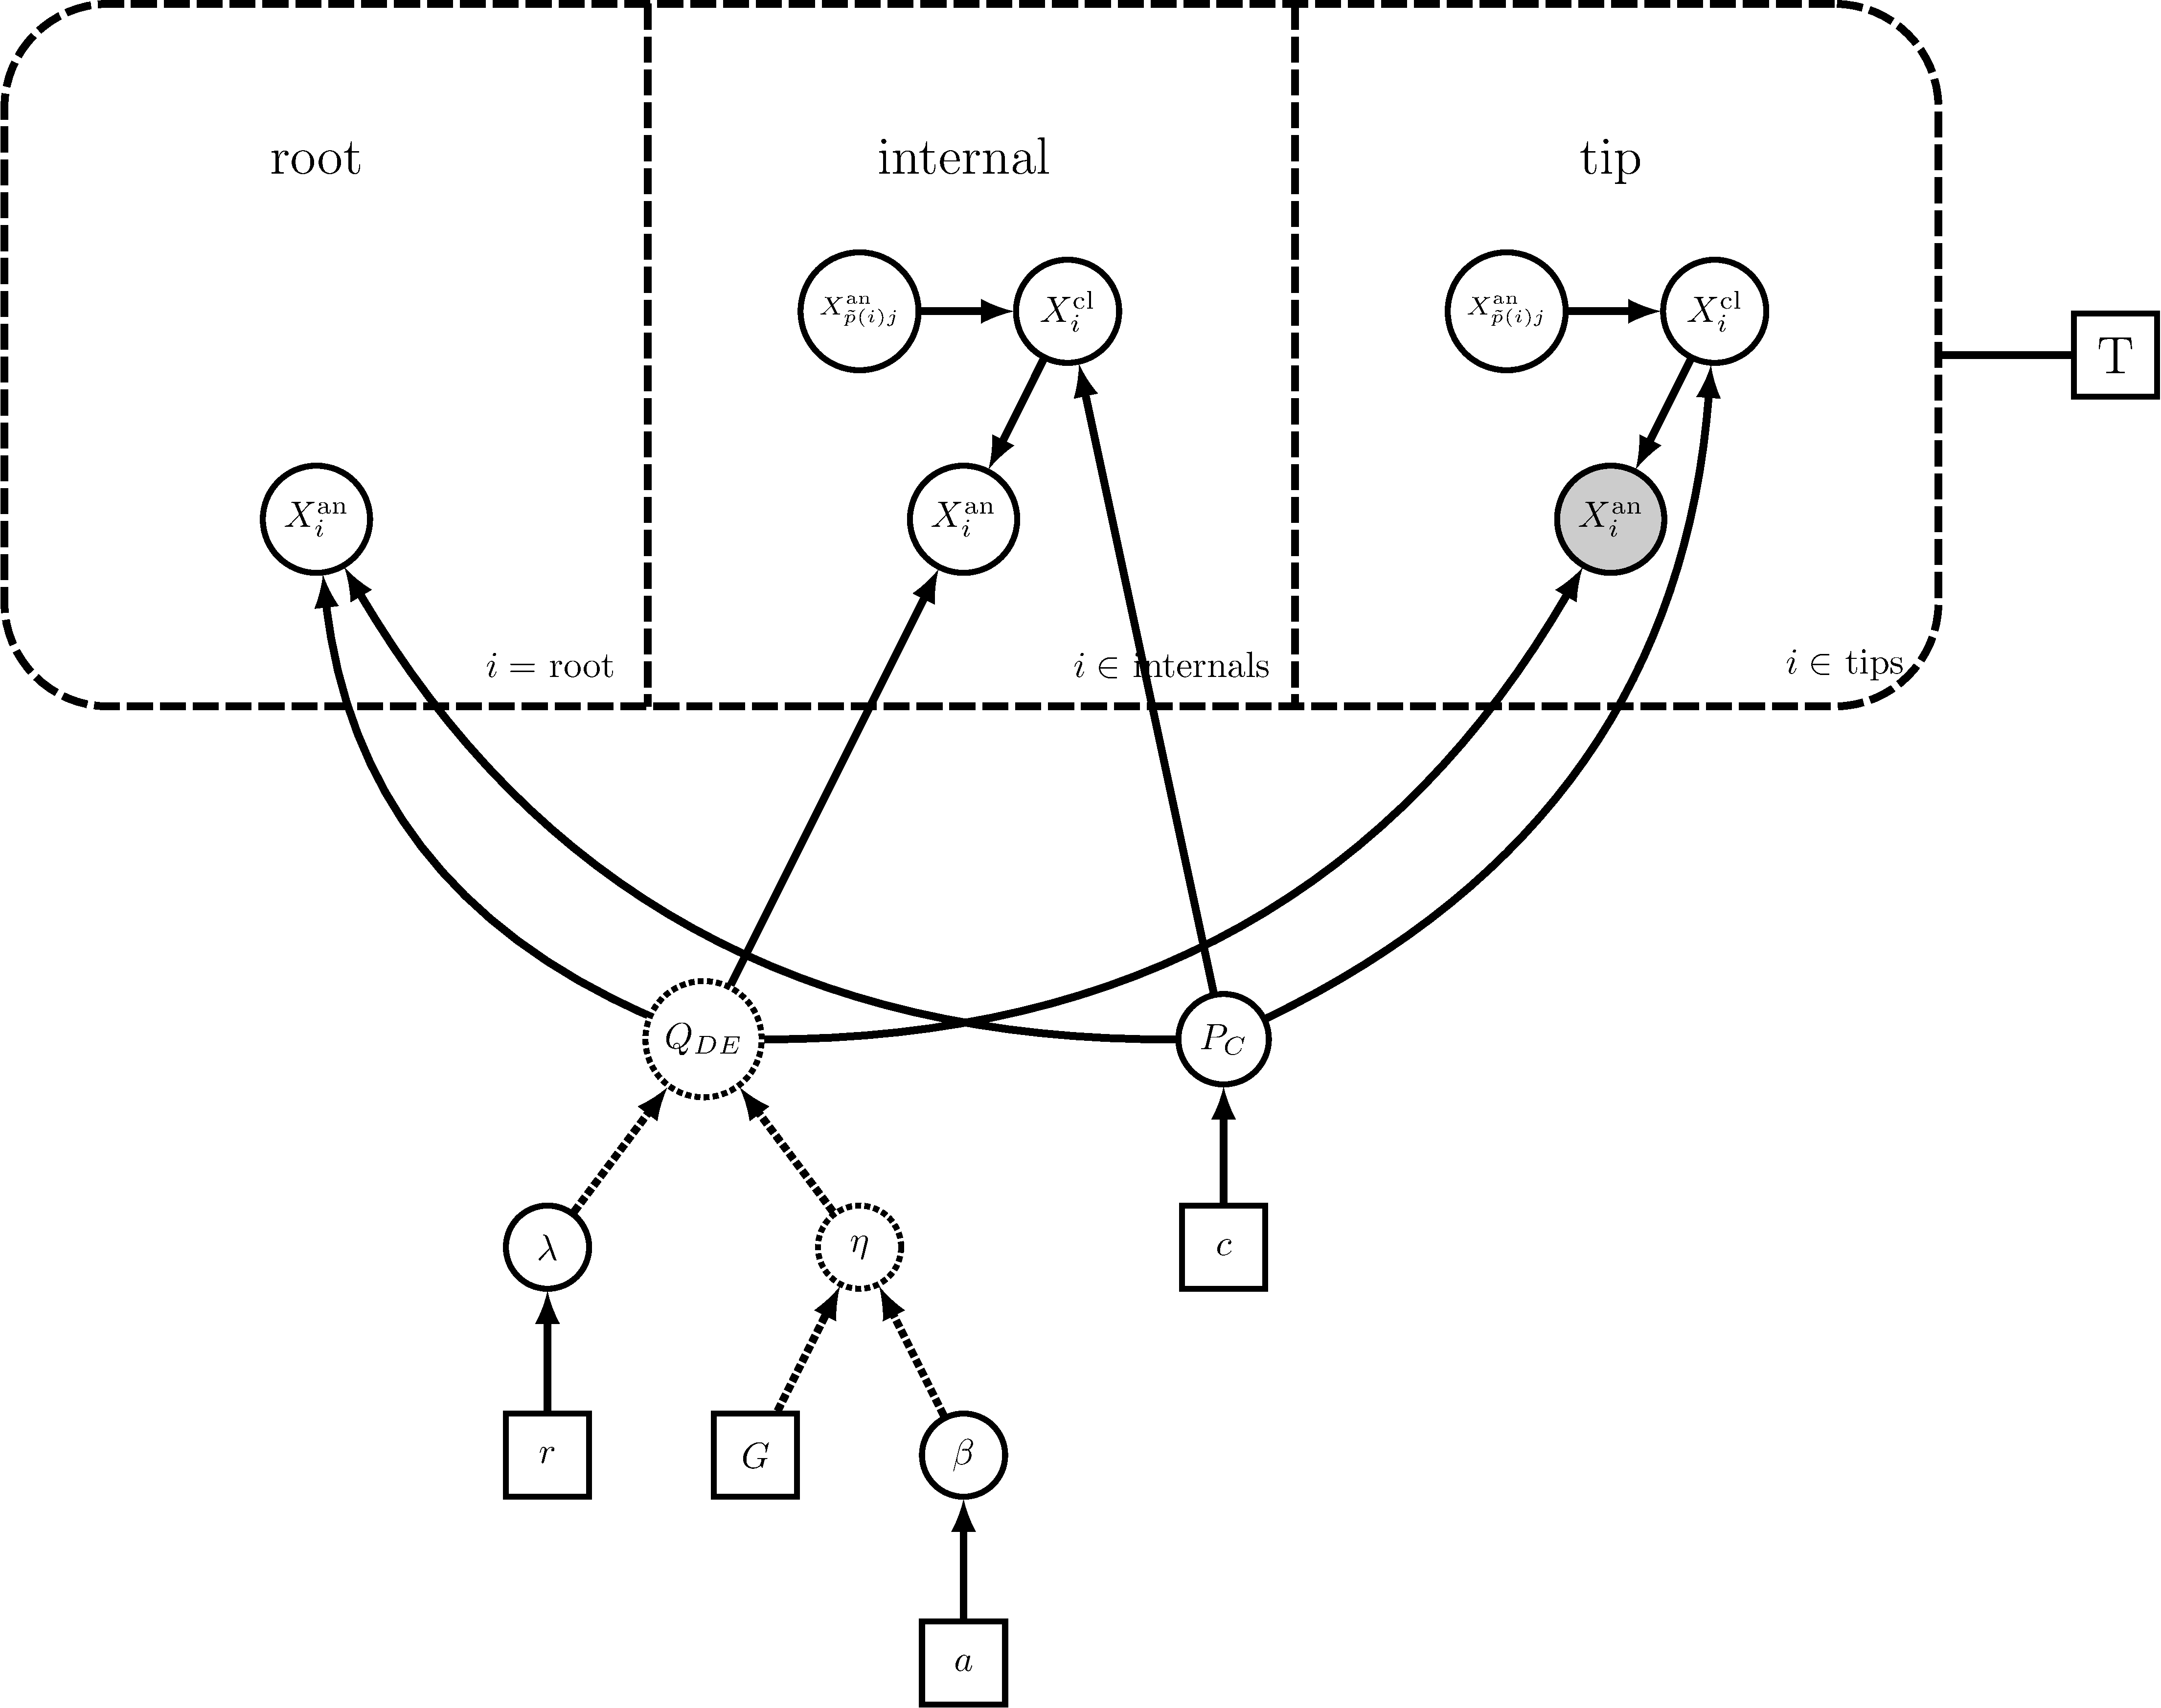
\includegraphics[width=5in]{figures/bg_dec_dag}
%\caption{Graphical model of DEC. The tree plate's topology is fixed by $T$, where each internal node has both an anagenic and cladogenic random variable ($X_i^{\text{an}}$ and $X_i^{\text{cl}}$, resp.) that represents an ancestral species before and after it speciated. Anagenic change is modeled by a continuous time Markov process, where $Q_{DE}$ is the instantaneous rate matrix of area gain and loss, as parameterized by $\lambda$. The geographic distance rate modifier function, $\eta$, takes in the geographical distances and strata as $G$, and the distance power parameter, $\beta$. Cladogenic change is modeled by $P_C$, a Dirichlet-distributed simplex with a flat prior.}
%\end{figure}

The rest of this section will describe how to run a simple DEC analysis using RevBayes.

\newpage

%%%%%%%%%%%%%%%%
%%%%%%%%%%%%%%%%

\subsubsection{Specifying a simple DEC model}

We'll use the primate dataset with 23 taxa. To keep the model simple, we'll discretize their ranges into just three areas: the New World (A), Africa (B), and Eurasia (C).
For simplicity, we'll assume their phylogeny is time-calibrated, errorless, and fixed.

Create some {\tt String} variables for file handling,
{\tt \small \begin{snugshade}
\begin{lstlisting}
data_fn = "data/primates_bg_n3.tsv"
tree_fn = "data/primates.tree"
out_fn  = "output/bg_same"
\end{lstlisting}
\end{snugshade} }

then read in our character data, using {\tt type="Bitset"} to indicate ranges are encoded with bits, e.g. 011

\begin{snugshade}
\begin{lstlisting}
data = readCharacterDataDelimited(file=data_fn, type="Bitset")
\end{lstlisting}
\end{snugshade}

and our tree

\begin{snugshade}
\begin{lstlisting}
psi <- readTrees(tree_fn)[1]
\end{lstlisting}
\end{snugshade}

Next, compute the number of states from the number of areas

\begin{snugshade}
\begin{lstlisting}
n_areas = 3
n_states = floor(2^n_areas)
\end{lstlisting}
\end{snugshade}

Declare index variables for our move vectors for future use

\begin{snugshade}
\begin{lstlisting}
mi = 0
\end{lstlisting}
\end{snugshade}

Now, we'll begin to construct the rate matrix for anagenic events. First create a matrix, 8-by-8 in size, initialized with all zeroes

\begin{snugshade}
\begin{lstlisting}
for (i in 1:n_states) {
    for (j in 1:n_states) {
        r[i][j] <- 0.0
    }
}
\end{lstlisting}
\end{snugshade}

Now we need to populate the non-zero rate matrix elements, which are in terms of dispersal and extinction rates.
We'll use one dispersal rate and one extinction rate for this tutorial, and explore more complex models in later sections.
For later reference, this will be called the ``same rate'' model.

First, create a extinction rate parameter and assign it a scale move

\begin{snugshade}
\begin{lstlisting}
r_e ~ dnExponential(10.0)
mv[++mi] = mvScale(r_e, weight=5)
\end{lstlisting}
\end{snugshade}

Before assigning the rates to the rate matrix, we'll create a vector to hold the per-area extinction rates 

\begin{snugshade}
\begin{lstlisting}
for (i in 1:n_areas) {
    e[i] := r_e
}
\end{lstlisting}
\end{snugshade}

Now create the dispersal rate and scale move

\begin{snugshade}
\begin{lstlisting}
r_d ~ dnExponential(10.0)
mv[++mi] = mvScale(r_d, weight=5)
\end{lstlisting}
\end{snugshade}

then assign the between-area dispersal rates as determined by {\tt $r_d$}

\begin{snugshade}
\begin{lstlisting}
for (i in 1:n_areas) {
    for (j in 1:n_areas) {
    	d[i][j] <- 0.
        if (i != j) {
            d[i][j] := r_d
        }
    }
}
\end{lstlisting}
\end{snugshade}

Although the DEC rate matrix can be easily constructed by typing

\begin{snugshade}
\begin{lstlisting}
q := fnDECRateMatrix(d,e)
\end{lstlisting}
\end{snugshade}

manually encoding the structure of the DEC rate matrix illuminates the relationship between dispersal rates, extinction rates, area gain rates, and area loss rates.
To start, we'll populate the non-zero rate matrix elements.
Rates are indexed by the natural number value of the range (plus one), e.g. the range spanning Eurasia and Africa is coded as 011, which is state 4.

First assign the extinction (range loss) rates

\begin{snugshade}
\begin{lstlisting}
r[2][1] := e[1]               # 100 -> 000 : Extirpate in area 1
r[3][1] := e[2]               # 010 -> 000 : Extirpate in area 2
r[4][2] := e[2]               # 011 -> 001 : Extirpate in area 2
r[4][3] := e[3]               # 011 -> 010 : Extirpate in area 3
r[5][1] := e[3]               # 001 -> 000 : Extirpate in area 3
r[6][2] := e[1]               # 101 -> 001 : Extirpate in area 1
r[6][5] := e[3]               # 101 -> 100 : Extirpate in area 3
r[7][3] := e[1]               # 110 -> 010 : Extirpate in area 1
r[7][5] := e[2]               # 110 -> 100 : Extirpate in area 2
r[8][4] := e[1]               # 111 -> 011 : Extirpate in area 1
r[8][6] := e[2]               # 111 -> 101 : Extirpate in area 2
r[8][7] := e[3]               # 111 -> 110 : Extirpate in area 3
\end{lstlisting}
\end{snugshade}

then the dispersal (range gain) rates

\begin{snugshade}
\begin{lstlisting}
r[2][4] := d[3][2]              # 001 -> 011 : Disperse from area 3 to 2
r[2][6] := d[3][1]              # 001 -> 101 : Disperse from area 3 to 1
r[3][4] := d[2][3]              # 010 -> 011 : Disperse from area 2 to 3
r[3][7] := d[2][1]              # 010 -> 110 : Disperse from area 2 to 1
r[5][6] := d[1][3]              # 100 -> 101 : Disperse from area 1 to 3
r[5][7] := d[1][2]              # 100 -> 110 : Disperse from area 1 to 2
r[4][8] := d[2][1] + d[3][1]  # 011 -> 111 : Disperse from area 2 to 1 and from 3 to 1
r[6][8] := d[1][2] + d[3][2]  # 101 -> 111 : Disperse from area 1 to 2 and from 3 to 2
r[7][8] := d[1][3] + d[2][3]  # 110 -> 111 : Disperse from area 1 to 3 and from 2 to 3
\end{lstlisting}
\end{snugshade}

Show the value of {\tt r} and compare it to the matrix in Section 2.2.

Of course we did not need to declare {\tt d} and {\tt e} to assign {\tt r}, but we'll see these intermediate variables act as a template expose the structure of {\tt r} for modification.

So far, we only have the desired parameterization of the rate matrix, but we still haven't created a rate matrix function. Converting the vector-of-vectors, {\tt r}, into a simplex allows us to use existing rate matrix functions. 

First, we'll convert {\tt r} into a one-dimensional vector, skipping the diagonal elements.

\begin{snugshade}
\begin{lstlisting}
k = 1
for (i in 1:n_states) {
    for (j in 1:n_states) {
        if (i != j) {
            er_nat[k++] := r[i][j]
        }
    }
}
\end{lstlisting}
\end{snugshade}

Finally, normalize {\tt er\_nat} using a simplex, then pass the resulting exchangeability rates as arguments into the rate matrix function, {\tt q}.

\begin{snugshade}
\begin{lstlisting}
er := simplex(er_nat)
bf <- simplex(rep(1,n_states))
q := fnFreeK(er, bf)
\end{lstlisting}
\end{snugshade}

This yields the desired three-area DEC rate matrix modeling anagenic character change.


In contrast, cladogenic event probabilites are given by a transition probability matrix and do not require a rate matrix.
First, we will create a vector of prior weights on cladogenesis events. Here, we assign a flat prior to all cladogenic events

\begin{snugshade}
\begin{lstlisting}
widespread_sympatry_wt <- 1.0
subset_sympatry_wt     <- 1.0
allopatry_wt           <- 1.0
clado_prior            <- [ widespread_sympatry_wt, subset_sympatry_wt, allopatry_wt ]
\end{lstlisting}
\end{snugshade}

then create the distribution over cladogenic event types and add its MCMC move

\begin{snugshade}
\begin{lstlisting}
clado_type             ~ dnDirichlet(clado_prior)
mv[++mi]               = mvSimplexElementScale(clado_type, alpha=10, weight=5)
\end{lstlisting}
\end{snugshade}

To give the simplex elements descriptive names when monitored, assign the values to deterministic nodes

\begin{snugshade}
\begin{lstlisting}
widespread_sympatry    := clado_type[1]
subset_sympatry        := clado_type[2]
allopatry              := clado_type[3]
\end{lstlisting}
\end{snugshade}

Then create the cladogenic transition probability matrix, which assigns probabilities to cladogenic event classes accoridng to {\tt clado\_type\_prob}

\begin{snugshade}
\begin{lstlisting}
clado_prob := fnCladoProbs(clado_type, n_areas, 2)
\end{lstlisting}
\end{snugshade}

Add a parameter for a biogeographical clock, which scales the overall rate of range evolution.
As a prior, an exponential distribution with rate 10 generates one dispersal or extinction event per 10 million years.

\begin{snugshade}
\begin{lstlisting}
clock_bg ~ dnExponential(10)
mv[++mi] = mvScale(clock_bg, weight=5)
\end{lstlisting}
\end{snugshade}

Finally, all our model components are encapsulated in the {\tt dnPhyloCTMCClado} distribution, which is similar to {\tt dnPhyloCTMC} except specialized to integrate over cladogenic events. Although this dataset has three areas, it is recognized single character with states valued from 1 to $2^3$, hence {\tt nSites=1}.

\begin{snugshade}
\begin{lstlisting}
m ~ dnPhyloCTMCClado( tree=psi, Q=q, cladoProbs=clado_prob, branchRates=clock_bg, nSites=1, type="NaturalNumbers" )
\end{lstlisting}
\end{snugshade}

The remaining tasks should be familiar by now, so we can proceed briskly. Attach the observed ranges to the model.

\begin{snugshade}
\begin{lstlisting}
m.clamp(data)
\end{lstlisting}
\end{snugshade}

Compose the model.

\begin{snugshade}
\begin{lstlisting}
mdl = model(m)
\end{lstlisting}
\end{snugshade}

Add the monitors. (The {\tt mnJointConditionalAncestralState} monitor will be described in the next section.)

\begin{snugshade}
\begin{lstlisting}
mn[1] = mnScreen(clock_bg, d[1][2], d[1][3], d[2][1], d[2][3], d[3][1], d[3][2], e[1], e[2], e[3], widespread_sympatry, subset_sympatry, allopatry, printgen=1000)
mn[2] = mnFile(clock_bg, d[1][2], d[1][3], d[2][1], d[2][3], d[3][1], d[3][2], e[1], e[2], e[3], widespread_sympatry, subset_sympatry, allopatry, file=out_fn+".params.txt")
mn[3] = mnJointConditionalAncestralState(tree=psi, ctmc=m, filename=out_fn+".states.txt", type="NaturalNumbers", printgen=10, withTips=true, withStartStates=true)
\end{lstlisting}
\end{snugshade}

Create the MCMC object, and run the chain after burn-in.
\begin{snugshade}
\begin{lstlisting}
ch = mcmc(mv,mn,mdl)
ch.burnin(1000, 10)
ch.run(10000)
\end{lstlisting}
\end{snugshade}

\subsubsection{Per-area rates}

Biologically, local extinction events probably do not occur at equal rates across all areas, as done above.
Ecological factors, geographical distances, etc. might cause these parameters to be weakly correlated or completely uncorrelated.
Dispersal rates, also, might not be the same between pairs of areas, or even symmetric depending on the direction of dispersal.
Rather than constraining all events of a type to share a common rate, instead you might give each area it's own extinction parameter

\begin{snugshade}
\begin{lstlisting}
for (i in 1:3) {
    e[i] ~ dnExponential(10.0)
    mv[++mi] = mvScale(e[i], weight=5)
}
\end{lstlisting}
\end{snugshade}

or give each ordered pair of areas it's own dispersal rate

\begin{snugshade}
\begin{lstlisting}
for (i in 1:3) {
    for (j in 1:3) {
    	d[i][j] <- 0.0
        if (i != j) {
            d[i][j] ~ dnExponential(10.0)
            mv[++mi] = mvScale(d[i][j], weight=5)
        }
    }
}
\end{lstlisting}
\end{snugshade}
Note that you don't need the global dispersal rate \cl{r\_d} and extinction rate \cl{r\_e} anymore and you can remove the variable from your analysis. \RevBayes~might give you an error message if you have left them in.

\subsection{Exercises}

Exercises are independent of each other, except for Exercises 3a and 3b.

\begin{itemize}
\item 1) Widespread sympatric speciation is thought to be evolutionarily rare. Set the Dirichlet prior on cladogenic event types to heavily disfavor these events. Using Tracer, describe how changing the cladogenesis prior affects the extinction rate when compared with the ``common rate'' model.
\item 2) Modifying the \RevBayes~script, parameterize the rate matrix so ranges may not grow beyond two areas in size. You may use {\tt q\_test := fnDECRateMatrix(e,d,2)} to confirm your results, which will give the same rate structure (and rates, up to a rescaling constant).
\item 3a) Saving your commands to a file, create a script to produce the ``per-area rate'' model.
\item 3b) Determine if the data support the ``common rate'' model over the ``per-area rate'' model. Use the stepping stone method to compute marginal likelihoods, which will let you compute Bayes factors for model selection.
%\item 4) (Advanced) Using what you learned in this tutorial and the CTMC tutorial, perform a joint analysis of molecular and biogeographic evolution for primates. Introduce a common prior for the molecular and biogeographical clocks, e.g.
%\begin{snugshade}
%\begin{lstlisting}
%clock_mol       ~ dnExponential(10.0)
%clock_scale_bg  ~ dnGamma(2.0,2.0)
%clock_bg        := clock_mol * clock_scale_bg
%\end{lstlisting}
%\end{snugshade}
\end{itemize}

\subsection{(Advanced) Joint inference of phylogeny and historical biogeography}
This is a slightly more advanced question that you may want to skip if you will always use known, fixed trees in your analyses.
Using what you learned in this tutorial and the CTMC tutorial, perform a joint analysis of molecular and biogeographic evolution for primates. 

Start by loading the sequence data matrix specified in \cl{data/primates\_cytb.nex}.
{\tt \begin{snugshade*}
\begin{lstlisting}
seqData <- readDiscreteCharacterData("data/primates_cytb.nex")
\end{lstlisting}
\end{snugshade*}}

We need to get some useful variables from the data so that we will be able to specify the tree prior below. These variables are the number of tips, the number of nodes and the names of the species which we all can query from the continuous character data object.
{\tt \small \begin{snugshade*}
\begin{lstlisting}
numTips = seqData.ntaxa()
names = seqData.names()
numNodes = numTips * 2 - 1
\end{lstlisting}
\end{snugshade*}}

Instead of having a fixed tree as in the previous, we should now define a \emph{random} tree. We use a birth death prior with prior distributions on the \cl{speciation} rate and \cl{extinction} rate.
{\tt \small \begin{snugshade*}
\begin{lstlisting}
speciation ~ dnExponential(10.)
extinction ~ dnExponential(10.)
moves[++mi] = mvScale(speciation, lambda=1, tune=true, weight=3.0)
moves[++mi] = mvScale(extinction, lambda=1, tune=true, weight=3.0)
\end{lstlisting}
\end{snugshade*}}
The phylogeny that we used are obviously not a complete sample of all the species and you should take the incomplete sampling into account. We will simply use an empirical estimate of the fraction of species which we included in this study. For more information about incomplete taxon sampling see \cite{Hohna2011} and \cite{Hohna2014a}. 
{\tt \small \begin{snugshade*}
\begin{lstlisting}
sampling_fraction <- 23 / 270     # 23 out of the ~ 270 primate species
\end{lstlisting}
\end{snugshade*}}
Now we are able to specify of tree variable \cl{psi} which is drawn from a constant rate birth-death process. We will condition the age of the tree to be 75 million years old which is approximately the crown age of primates, although this estimate is still debated. We only condition here on the crown age for simplicity because we do not use any other fossil calibration.
{\tt \small \begin{snugshade*}
\begin{lstlisting}
psi ~ dnBDP(lambda=speciation, mu=extinction, rho=sampling_fraction, rootAge=75, nTaxa=numTips, names=names)
\end{lstlisting}
\end{snugshade*}}
Note that, here, we do not have included any fossil information: we are merely doing \emph{relative} dating. 

The first moves on the tree which we specify are moves that change the node ages. The first move randomly picks a subtree and rescales it, and the second move randomly pick a node and uniformly proposes a new node age between its parent age and oldest child's age.
{\tt \small \begin{snugshade*}
\begin{lstlisting}
moves[++mi] = mvSubtreeScale(psi, weight=5.0)
moves[++mi] = mvNodeTimeSlideUniform(psi, weight=10.0)
\end{lstlisting}
\end{snugshade*}}

We also need moves on the tree topology to estimate the phylogeny. The two moves which you use are the nearest-neighbor interchange (NNI) and the fixed-nodeheight-prune-and-regraft (FNPR) \citep{Hohna2012}.
{\tt \small \begin{snugshade*}
\begin{lstlisting}
moves[++mi] = mvNNI(psi, weight=5.0)
moves[++mi] = mvFNPR(psi, weight=5.0)\end{lstlisting}
\end{snugshade*}}


In the next step we set up the substitution model.
First, we create a substitution model, just like what you probably did in previous tutorial (\EG RB\_CTMC\_Tutorial). 
In a first step, we will use a GTR+Gamma model.
We can use a flat Dirichlet prior density on the exchangeability rates \cl{er\_mol} and the the base frequencies \cl{pi\_mol}.
{\tt \begin{snugshade*}
\begin{lstlisting}
er_mol_prior <- v(1,1,1,1,1,1) 
er_mol ~ dnDirichlet(er_mol_prior)
pi_mol_prior <- v(1,1,1,1) 
pi_mol ~ dnDirichlet(pi_mol_prior)
\end{lstlisting}
\end{snugshade*}}
Now add the simplex scale move one each the exchangeability rates \cl{er\_mol} and the stationary frequencies \cl{pi\_mol} to the moves vector:
{\tt \small \begin{snugshade*}
\begin{lstlisting}
moves[++mi] = mvSimplexElementScale(er_mol,weight=15) 
moves[++mi] = mvSimplexElementScale(pi_mol,weight=5)  
\end{lstlisting}
\end{snugshade*}}
We can finish setting up this part of the model by creating a deterministic node for the GTR instantaneous-rate matrix \cl{Q\_mol}. 
The \cl{fnGTR()} function takes a set of exchangeability rates and a set of base frequencies to compute the instantaneous-rate matrix used when calculating the likelihood of our model.
{\tt \begin{snugshade*}
\begin{lstlisting}
Q_mol := fnGTR(er_mol,pi_mol)
\end{lstlisting}
\end{snugshade*}}
The next part of the substitution process is the rate variation among sites. We will model this using the commonly applied 4 discrete gamma categories which only have a single parameter \cl{alpha}.
Let us specify the rate of \cl{alpha} to 0.05 (thus the mean will be 20.0).
{\tt\begin{snugshade*}
\begin{lstlisting}
alpha_prior <- 0.05                                                                             
\end{lstlisting}
\end{snugshade*}}
Then create a stochastic node called \cl{alpha} with an exponential prior:
{\tt\begin{snugshade*}
\begin{lstlisting}
alpha ~ dnExponential(alpha_prior)
\end{lstlisting}
\end{snugshade*}}
Initialize the \cl{gamma\_rates} deterministic node vector using the  \cl{fnDiscretizeGamma()} function with \cl{4} bins:
{\tt \begin{snugshade*}
\begin{lstlisting}
gamma_rates := fnDiscretizeGamma( alpha, alpha, 4 )
\end{lstlisting}
\end{snugshade*}}
The random variable that controls the rate variation is the stochastic node \cl{alpha}. 
We will apply a simple scale move to this parameter.
{\tt \begin{snugshade*}
\begin{lstlisting}
moves[++mi] = mvScale(alpha, weight=2.0)
\end{lstlisting}
\end{snugshade*}}
This finishes the substitution process part of the model.

Then next part of the model is the clock model. Here we need a clock model because we work on a time tree. We use an exponential distribution with expectation 0.1.
{\tt \begin{snugshade*}
\begin{lstlisting}
clock_mol ~ dnExponential(10)
moves[++mi] = mvScale(clock_mol, lambda=1, tune=true, weight=2.0)
\end{lstlisting}
\end{snugshade*}}

Introduce a common prior for the molecular and biogeographical clocks.
\begin{snugshade}
\begin{lstlisting}
clock_scale_bg  ~ dnGamma(2.0,2.0)
clock_bg        := clock_mol * clock_scale_bg
\end{lstlisting}
\end{snugshade}

Remember that you need to call the \cl{PhyloCTMC} constructor to include the new site-rate parameter:

{\tt \begin{snugshade*}
\begin{lstlisting}
seq ~ dnPhyloCTMC(tree=psi, Q=Q_mol, siteRates=gamma_rates, branchRates=clockRate, type="DNA")
\end{lstlisting}
\end{snugshade*}}
Finally we need to attach the molecular sequence data to our model.
{\tt \begin{snugshade*}
\begin{lstlisting}
seq.clamp(seqData)
\end{lstlisting}
\end{snugshade*}}

We are essentially done now. We  only need to add a new monitor for the tree so that we can monitor and build the maximum a posteriori tree later.
{\tt \small \begin{snugshade*}
\begin{lstlisting}
monitors[3] = mnFile(filename="output/biogeography_DEC_joint.trees", printgen=100, separator = TAB, psi)
\end{lstlisting}
\end{snugshade*}}

Create the range evolution model as before, being sure to use the same {\tt psi} and {\tt clock\_bg} from above.

The remaining challenge is to compose both submodels together using {\tt model} and creating an MCMC object with {\tt mcmc}. Good luck!

\newpage
